\documentclass[12pt]{article}
%\usepackage[utf8]{inputenc}
%\documentclass[UTF8]{ctexart}
%\usepackage[UTF8, heading = false, scheme = plain]{ctex}
\usepackage{geometry}
%geometry{a4paper,scale=0.9}
\geometry{a4paper,left=1cm,right=1cm,top=1cm,bottom=2cm}
\usepackage{amsfonts}
\usepackage{color}
\usepackage{url}
%\usepackage{biblatex}
\usepackage{amsmath}
\usepackage{amssymb}
\usepackage{latexsym}
\usepackage{listings}
\usepackage[usenames,dvipsnames]{xcolor}
\usepackage{cite}
%\addbibresource{ref.bib}
%\bibliography{ref.bib}
\usepackage{caption}
\usepackage{graphicx, subfig}
\usepackage{float}
%\usepackage[fontset=ubuntu]{ctex}
%\usepackage{fontspec}
\usepackage{xeCJK}
%\usepackage[colorlinks,
%anchorcolor=black,
%citecolor=black]{hyperref}
%\setmainfont{SimSun}
\usepackage[section]{placeins}
\usepackage{enumitem}
\usepackage{framed}
\usepackage[framemethod=TikZ]{mdframed}
\usepackage{indentfirst}
\usepackage{setspace}%使用间距宏包
\linespread{1.5}
\definecolor{mygreen}{rgb}{0,0.6,0}
\definecolor{mygray}{rgb}{0.5,0.5,0.5}
\definecolor{mybgray}{rgb}{0.95,0.95,0.95}
\definecolor{mymauve}{rgb}{0.58,0,0.82}
\lstset{
 backgroundcolor=\color{mybgray}, 
 basicstyle = \footnotesize,       
 breakatwhitespace = false,        
 breaklines = true,                 
 captionpos = b,                    
 commentstyle = \color{mygreen}\bfseries,
 extendedchars = false,             
 frame =shadowbox, 
 framerule=0.5pt,
 keepspaces=true,
 keywordstyle=\color{blue}\bfseries, % keyword style
 language = C++,                     % the language of code
 otherkeywords={string}, 
 numbers=left, 
 numbersep=5pt,
 numberstyle=\tiny\color{mygray},
 rulecolor=\color{black},         
 showspaces=false,  
 showstringspaces=false, 
 showtabs=false,    
 stepnumber=1,         
 stringstyle=\color{mymauve},        % string literal style
 tabsize=2,          
 title=\lstname                      
}

\title{图相关}
\author{leolinuxer}
%\date{June 2020}

\begin{document}
%\setlength{\parindent}{0pt}
\maketitle
\tableofcontents

\section{二分图}
\url{https://github.com/labuladong/fucking-algorithm/blob/master/%E7%AE%97%E6%B3%95%E6%80%9D%E7%BB%B4%E7%B3%BB%E5%88%97/%E4%B8%BA%E4%BB%80%E4%B9%88%E6%8E%A8%E8%8D%90%E7%AE%97%E6%B3%954.md}

简单来说,二分图就是一幅拥有特殊性质的图:能够用两种颜色为所有顶点着色,使得任何一条边的两个顶点颜色不同。
\begin{figure}[H]
    \centering
    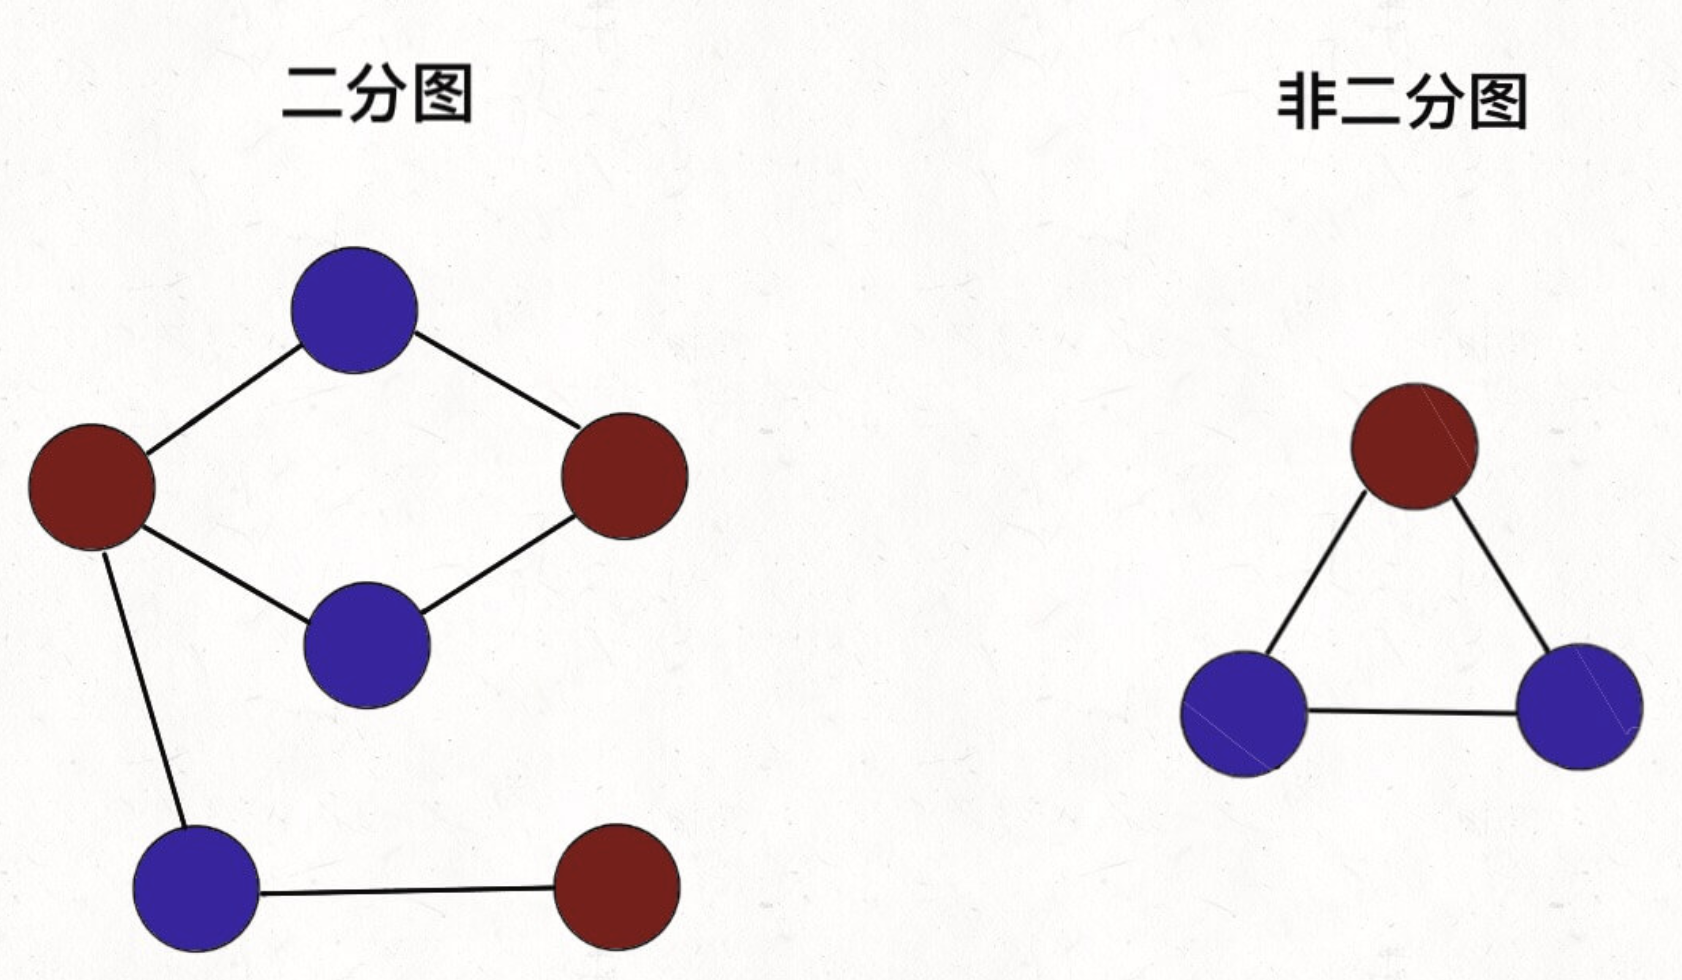
\includegraphics[width=.5\textwidth]{fig/FA_BiGraph_1.png}
\end{figure}

明白了二分图是什么,能解决什么实际问题呢?\textbf{算法方面,常见的操作是如何判定一幅图是不是二分图}。比如说下面这道 LeetCode 题目:
\begin{figure}[H]
    \centering
    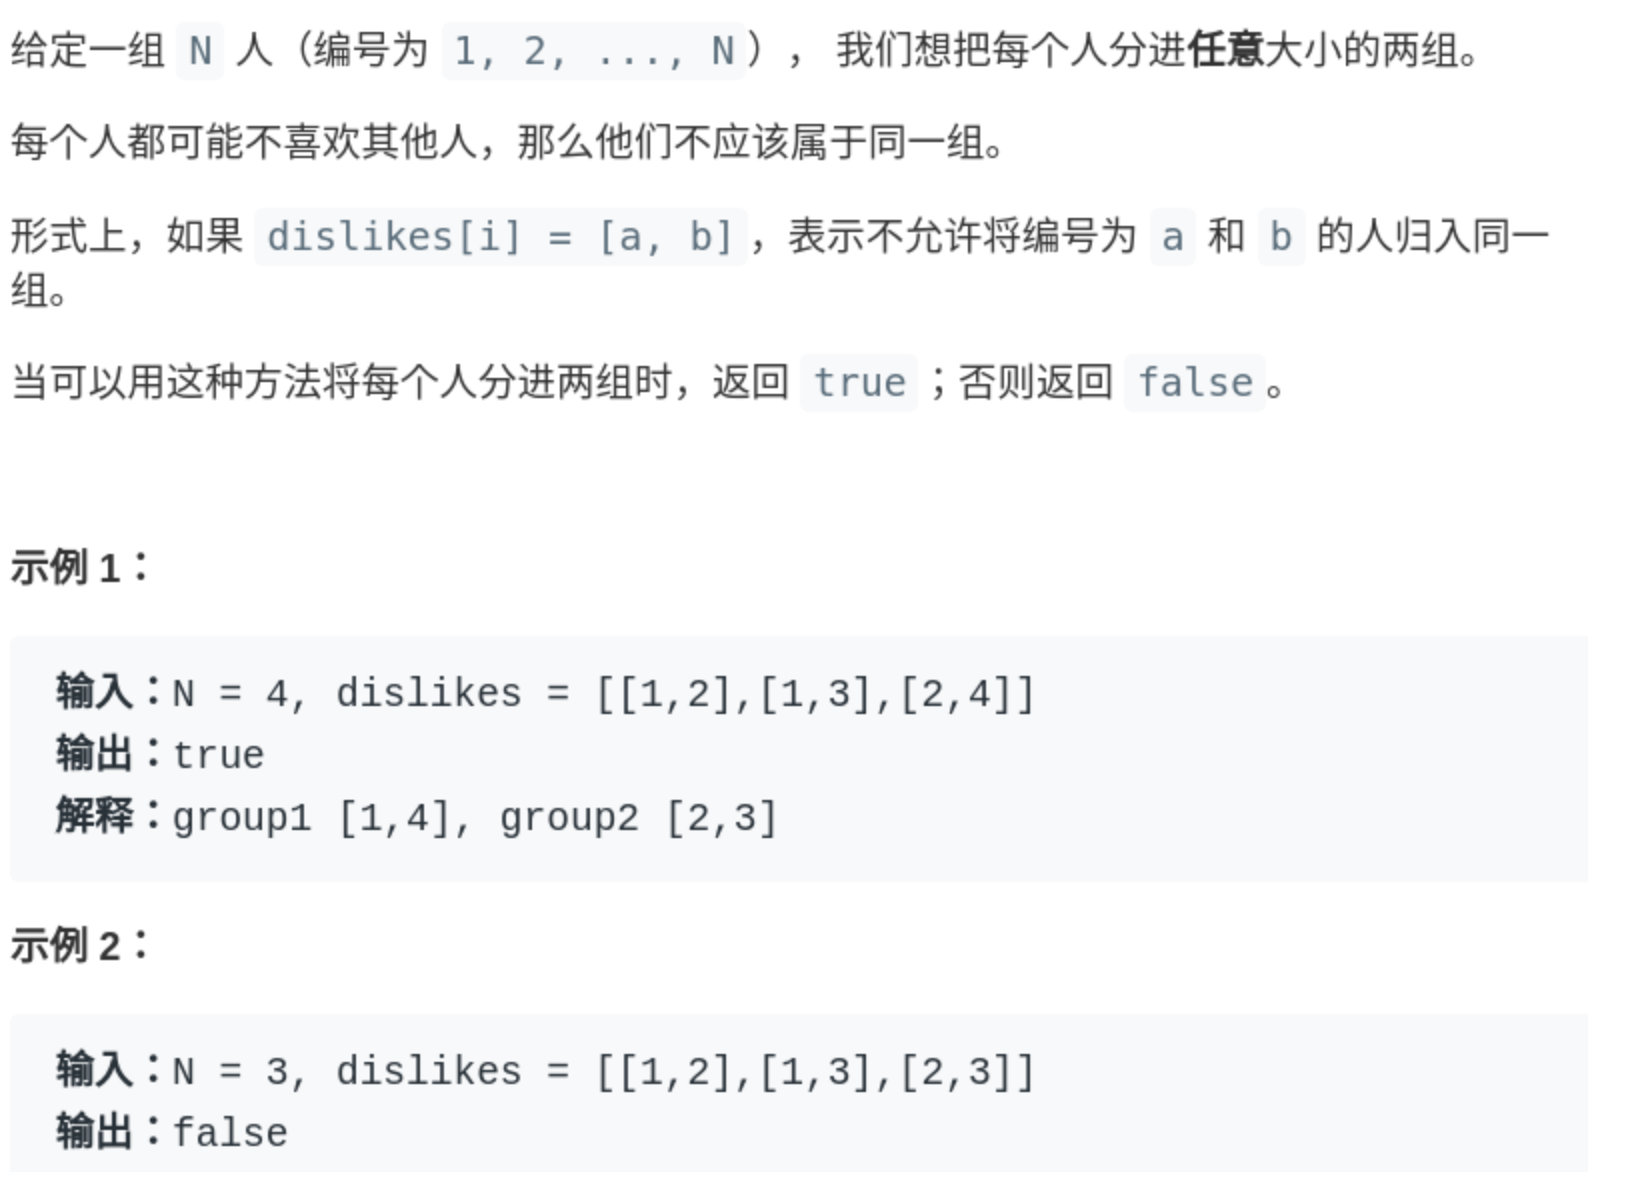
\includegraphics[width=.8\textwidth]{fig/FA_BiGraph_2.png}
\end{figure}

如果我们把每个人视为一个顶点,边代表讨厌;相互讨厌的两个人之间连接一条边,就可以形成一幅图。那么根据刚才二分图的定义,如果这幅图是一幅二分图,就说明这些人可以被分为两组,否则的话就不行。

这是判定二分图算法的一个应用,其实二分图在数据结构方面也有一些不错的特性。

比如说我们需要一种数据结构来储存电影和演员之间的关系:某一部电影肯定是由多位演员出演的,且某一位演员可能会出演多部电影。你使用什么数据结构来存储这种关系呢?既然是存储映射关系,最简单的不就是使用哈希表嘛,我们可以使用一个 HashMap<String, List<String>> 来存储电影到演员列表的映射,如果给一部电影的名字,就能快速得到出演该电影的演员。

但是如果给出一个演员的名字,我们想快速得到该演员演出的所有电影,怎么办呢?这就需要「反向索引」,对之前的哈希表进行一些操作,新建另一个哈希表,把演员作为键,把电影列表作为值。

对于上面这个例子,可以使用二分图来取代哈希表。\textbf{电影和演员是具有二分图性质的}:如果把电影和演员视为图中的顶点,出演关系作为边,那么与电影顶点相连的一定是演员,与演员相邻的一定是电影,不存在演员和演员相连,电影和电影相连的情况。

如果这幅图构建完成,就不需要反向索引,对于演员顶点,其直接连接的顶点就是他出演的电影,对于电影顶点,其直接连接的顶点就是出演演员。


\section{相关题目}
\subsection{套汇的算法}
\url{https://github.com/labuladong/fucking-algorithm/blob/master/%E7%AE%97%E6%B3%95%E6%80%9D%E7%BB%B4%E7%B3%BB%E5%88%97/%E4%B8%BA%E4%BB%80%E4%B9%88%E6%8E%A8%E8%8D%90%E7%AE%97%E6%B3%954.md}

如果我们说货币 A 到货币 B 的汇率是 10,意思就是 1 单位的货币 A 可以换 10 单位货币 B。如果我们把每种货币视为一幅图的顶点,货币之间的汇率视为加权有向边,那么整个汇率市场就是一幅「完全加权有向图」。一旦把现实生活中的情景抽象成图,就有可能运用算法解决一些问题。比如说图中可能存在下面的情况:
\begin{figure}[H]
    \centering
    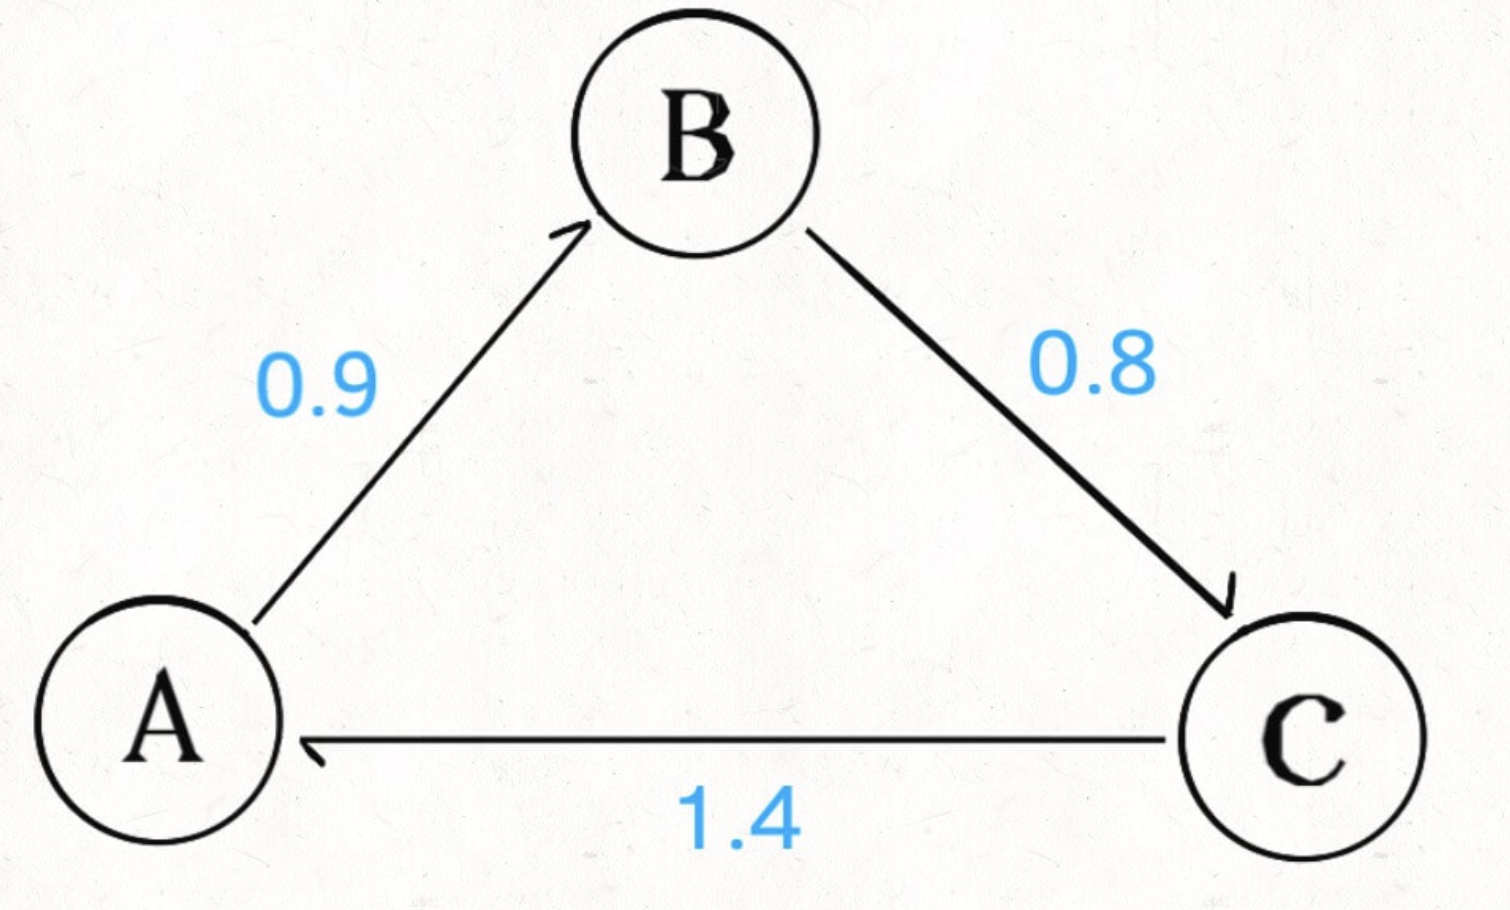
\includegraphics[width=.5\textwidth]{fig/FA_Graph_Problem_1.png}
\end{figure}
图中的加权有向边代表汇率,我们可以发现如果把 100 单位的货币 A 换成 B,再换成 C,最后换回 A,就可以得到 100×0.9×0.8×1.4 = 100.8 单位的 A!如果交易的金额大一些的话,赚的钱是很可观的,这种空手套白狼的操作就是套汇。

现实中交易会有种种限制,而且市场瞬息万变,但是套汇的利润还是很高的,关键就在于如何快速找到这种套汇机会呢?借助图的抽象,我们发现\textbf{套汇机会其实就是一个环,且这个环上的权重之积大于 1},只要在顺着这个环交易一圈就能空手套白狼。

图论中有一个经典算法叫做 Bellman-Ford 算法,可以用于寻找负权重环。对于我们说的套汇问题,可以\textbf{先把所有边的权重 w 替换成 -ln(w),这样「寻找权重乘积大于 1 的环」就转化成了「寻找权重和小于 0 的环」},就可以使用 Bellman-Ford 算法在 O(EV) 的时间内寻找负权重环,也就是寻找套汇机会。



%\printbibliography
\bibliography{../ref}
\bibliographystyle{IEEEtran}
\end{document}